%%% Uncomment the following for normal slide show
\documentclass[10pt,serif,professionalfont]{beamer}

%%% or uncomment this for handouts
% \documentclass[handout,ignorenonframetext]{beamer}

%%% or uncomment this for the article version
% \documentclass[11pt]{article}
% \usepackage{beamerarticle}

%%% Based on a TeXnicCenter-Template by Tino Weinkauf.
%%%%%%%%%%%%%%%%%%%%%%%%%%%%%%%%%%%%%%%%%%%%%%%%%%%%%%%%%%%%%

%\usepackage[utf8]{inputenc}
\usepackage[ansinew]{inputenc}

\usepackage[english]{babel}
%\usepackage[bibnewpage]{apacite}
%\usepackage{natbib}

\usepackage{fancyhdr}
\usepackage{setspace}
\usepackage{indentfirst}
\usepackage{booktabs}

\usepackage{amsmath, amsbsy, amssymb}

\usepackage{graphics}
\usepackage{graphicx}
\usepackage{subfig}
\usepackage{caption}
\usepackage{float}
\usepackage{rotating}
\usepackage{pdflscape}
\usepackage{caption}

\usepackage{soul} %for highlighting for mark?
\usepackage{color}
%\sethlcolor{white}




%%%%%%%%%%%%%%%%%%%%%%%%%%%%
%%% Beamer Stuff
%%%%%%%%%%%%%%%%%%%%%%%%%%%%

\let\Tiny=\tiny

\mode<article>
{
  \usepackage{fullpage}
  \usepackage{pgf}
  \usepackage{hyperref}
  \setjobnamebeamerversion{example.beamer}
}

\mode<presentation>
{
  % \usetheme{Dresden}
  % \usetheme{Marburg}
  % \usetheme{Hannover}
  \usetheme{Singapore}
  % \useoutertheme{smoothbars}
  % \useoutertheme{infolines}
  \usecolortheme{seagull}
  \setbeamercovered{invisible}
  \setbeamertemplate{navigation symbols}{}%remove navigation symbols
%  \setbeamertemplate{footline}[page number]
  \setbeamertemplate{footline}[frame number]
}

\mode<handout>
{
%%% In handout mode give the individual pages a light grey background
\setbeamercolor{background canvas}{bg=black!5}
%%% Put more than one frame on each page to save paper.
\usepackage{pgfpages}
\pgfpagesuselayout{4 on 1}[letterpaper,border shrink=3mm, landscape]
% \pgfpagesuselayout{2 on 1}[letterpaper,border shrink=5mm, portrait]
% \setbeameroption{show notes}
}
% \usepackage[latin1]{inputenc}

\setbeamertemplate{itemize items}[default]
\setbeamertemplate{enumerate items}[default]
\setbeamertemplate{frametitle continuation}[from second]

\setbeamercovered{transparent}

%\usepackage{appendixnumberbeamer}

\usepackage[T1]{fontenc}
\usepackage[osf]{mathpazo}
%\linespread{1.05}         % Palatino needs more leading (space between lines)

%\usepackage{pxfonts}
%\usepackage{eulervm}

 %David I didn't have access to this file!!!
%% Based on a TeXnicCenter-Template by Tino Weinkauf.
%%%%%%%%%%%%%%%%%%%%%%%%%%%%%%%%%%%%%%%%%%%%%%%%%%%%%%%%%%%%%

%\usepackage[utf8]{inputenc}
\usepackage[ansinew]{inputenc}

\usepackage[english]{babel}
%\usepackage[bibnewpage]{apacite}
%\usepackage{natbib}

\usepackage{fancyhdr}
\usepackage{setspace}
\usepackage{indentfirst}
\usepackage{booktabs}

\usepackage{amsmath, amsbsy, amssymb}

\usepackage{graphics}
\usepackage{graphicx}
\usepackage{subfig}
\usepackage{caption}
\usepackage{float}
\usepackage{rotating}
\usepackage{pdflscape}
\usepackage{caption}

\usepackage{soul} %for highlighting for mark?
\usepackage{color}
%\sethlcolor{white}




%%%%%%%%%%%%%%%%%%%%%%%%%%%%
%%% Beamer Stuff
%%%%%%%%%%%%%%%%%%%%%%%%%%%%

\let\Tiny=\tiny

\mode<article>
{
  \usepackage{fullpage}
  \usepackage{pgf}
  \usepackage{hyperref}
  \setjobnamebeamerversion{example.beamer}
}

\mode<presentation>
{
  % \usetheme{Dresden}
  % \usetheme{Marburg}
  % \usetheme{Hannover}
  \usetheme{Singapore}
  % \useoutertheme{smoothbars}
  % \useoutertheme{infolines}
  \usecolortheme{seagull}
  \setbeamercovered{invisible}
  \setbeamertemplate{navigation symbols}{}%remove navigation symbols
%  \setbeamertemplate{footline}[page number]
  \setbeamertemplate{footline}[frame number]
}

\mode<handout>
{
%%% In handout mode give the individual pages a light grey background
\setbeamercolor{background canvas}{bg=black!5}
%%% Put more than one frame on each page to save paper.
\usepackage{pgfpages}
\pgfpagesuselayout{4 on 1}[letterpaper,border shrink=3mm, landscape]
% \pgfpagesuselayout{2 on 1}[letterpaper,border shrink=5mm, portrait]
% \setbeameroption{show notes}
}
% \usepackage[latin1]{inputenc}

\setbeamertemplate{itemize items}[default]
\setbeamertemplate{enumerate items}[default]
\setbeamertemplate{frametitle continuation}[from second]

\setbeamercovered{transparent}

%\usepackage{appendixnumberbeamer}

\usepackage[T1]{fontenc}
\usepackage[osf]{mathpazo}
%\linespread{1.05}         % Palatino needs more leading (space between lines)

%\usepackage{pxfonts}
%\usepackage{eulervm}


\usepackage{outlines}
\usepackage{multirow}

\renewcommand*{\thefootnote}{\fnsymbol{footnote}}

\title{Applying the Axioms of Additive Conjoint Measurement to a Hierarchy of Latent Variable Models}

\author{Ronli Diakow\inst{1}\footnote[frame]{Authors are listed in alphabetical order.} \and Benjamin Domingue\inst{2}\footnotemark[1] \and David Torres Irribarra\inst{3}\footnotemark[1]}

\subject{Tenable Assessment}

\date{International Meeting of the Psychometric Society \\ July 25, 2013}

\institute[]{
  \inst{1} New York University \and 
  \inst{2} University of Colorado at Boulder \and
  \inst{3} University of California, Berkeley}

\begin{document}

\frame{\maketitle}

\section{Two methods}
\begin{frame}
    \frametitle{Score scales and latent structure}

    \begin{outline}
        \1 We want to adequately characterize psychological and educational variables. 
            \2 Are differences between respondents categorical?  ordered?  distances?  
            \2 How can we determine the (``correct'') generating model?  
        
        \vspace{0.25cm}    
        
        \1 This issue has both theoretical and practical importance.  
            \2 Foundation of many debates in policy and substantive research
            \2 Any decision matters for subsequent inferences
    \end{outline}
    
\end{frame}

\begin{frame}
    \frametitle{A tale of two methods}

    %love the title!  %thanks!

    \begin{outline}
        %\1 There have been a number of theoretical challenges regarding the possibility, in principle, of making this distinctions in psychometric (references).
        \1 Joint work based on two previous lines of research:
        \vspace{0.1cm}
            \2 Torres Irribarra and Diakow -- Can we determine the structure (qualitative, ordinal, interval) of a latent variable by model fit comparisons within a hierarchical model framework that places progressively more stringent monotonicity and scale assumptions on the latent variable?
            
            \vspace{0.25cm}
            
            \2 Domingue -- Do data possess sufficient structure, as judged by the axioms of conjoint measurement, to yield interval scales?
    \end{outline}

\end{frame}

%monotonicity and scale
\frame{

    \frametitle{Organizing models by their latent structure}

    Two kinds of restrictions that a model places on the latent variable:
    %(a) monotonicity and (b) scale.
    \begin{description}
        \item[\textbf{Monotonicity},] which implies that the probability a correct response is a non-decreasing function of increasing proficiency and/or is a non-increasing function of increasing difficulty.
        \item[\textbf{Scale},] which implies that the differences between persons (and items) are quantitative (i.e. interval) in nature.  
    \end{description}

}


\frame{

    \frametitle{A hierarchy of latent variable models}

        \centering 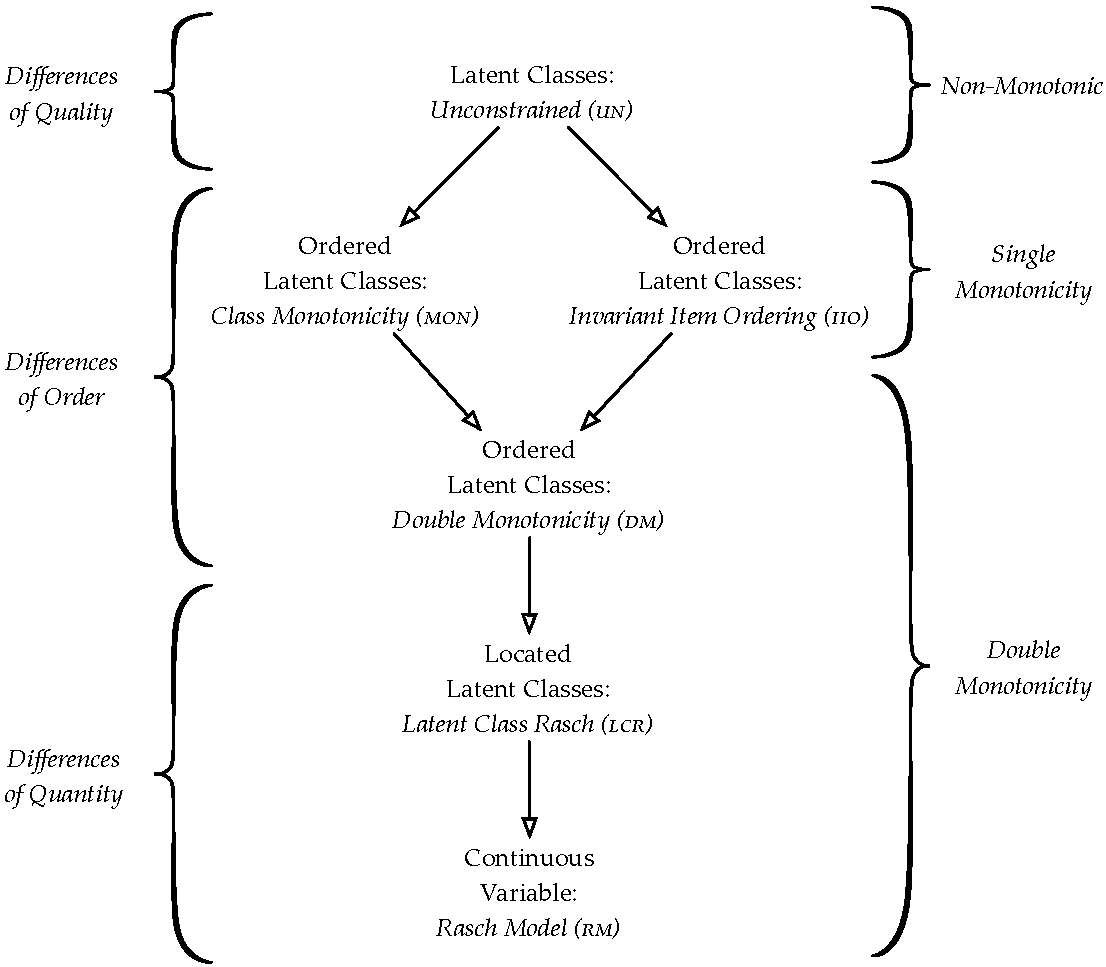
\includegraphics[width=0.75\textwidth]{./figs/Structure3.pdf} 

}


%models and equations
\frame[allowframebreaks]{

    \frametitle{Six latent variable models}

    \begin{enumerate}
    \parskip 9pt
        \item Unconstrained Latent Class Model (\textsc{un}):
            \begin{equation*} \label{eqn:lcabeta}
                \mathrm{logit} [ Pr(x_{ic} = 1 | c)] = \mathrm{logit} [\pi_{i|c}] = \beta_{ic}
            \end{equation*}

        \item Ordered Latent Class Model with Class Monotonicty (\textsc{mon}):
            \begin{eqnarray*} \label{eqn:monbeta}
               \mathrm{logit} [ Pr(x_{ic} = 1 | c)] = \mathrm{logit} [\pi_{i|c}] = \beta_{ic}, \\
               \beta_{ic} \leq \beta_{ic'} \mbox{ for all $c < c'$ and for all $i$} \nonumber
            \end{eqnarray*}

        \item Ordered Latent Class Model with Invariant Item Ordering (\textsc{iio}):
            \begin{eqnarray*} \label{eqn:iiobeta}
               \mathrm{logit} [ Pr(x_{ic} = 1 | c)] = \mathrm{logit} [\pi_{i|c}] = \beta_{ic}, \\
               \beta_{ic} \leq \beta_{i'c} \mbox{ for all $i < i'$ and for all $c$} \nonumber
            \end{eqnarray*}

        \item Ordered Latent Class Model with Double Monotonicity (\textsc{dm}):
            \begin{eqnarray*} \label{eqn:dmbeta}
               \mathrm{logit} [ Pr(x_{ic} = 1 | c)] = \mathrm{logit} [\pi_{i|c}] = \beta_{ic}, \\
               \beta_{ic} \leq \beta_{ic'} \mbox{ for all $c < c'$ and for all $i$} \nonumber, \\
               \beta_{ic} \leq \beta_{i'c} \mbox{ for all $i < i'$ and for all $c$} \nonumber
            \end{eqnarray*}

        \item Located Latent Class Model or Latent Class Rasch Model (\textsc{lcr}):
            \begin{equation*} \label{eqn:LCR}
                logit [ Pr(x_{ic} = 1 | \theta_c, \delta_i)] = \theta_c - \delta_i
            \end{equation*}

        \item Rasch Model (\textsc{rm}):
            \begin{equation*}
                \label{eqn:RSH}
                logit [ Pr(x_{ip} = 1 | \theta_p, \delta_i)] = \theta_p - \delta_i
            \end{equation*}
    \end{enumerate}

}


\begin{frame}
    \frametitle{Additive Conjoint Measurement (\textsc{acm})}

    % From Ben's abstract in Psychometrika:

    \begin{outline}
        \1 Axioms of additive conjoint measurement: 
            \2 Describe conditions that need to be satisfied for an interval scale to exist for an attribute
            \2 Provide a means of testing the hypothesis that data is consistent with an interval scale  
            \2 Are difficult to verify given (likely) measurement error  
            
        \vspace{0.25cm}
        
        \1 Focus on the cancelation axioms
    \end{outline}

\end{frame}

\begin{frame} 
    \frametitle{Cancelation axioms}
    
    Consider a $3 \times 3$ probability matrix formed by the selection of 3 item difficulties and 3 person abilities:
    \[
    \begin{array}{ccc}
      x_{11} & x_{12} & x_{13}  \\
      x_{21} & x_{22} & x_{23} \\
      x_{31} & x_{32} & x_{33} \\
    \end{array}
    \]
    
    \begin{outline}
        \1 Single cancelation: Rows or columns can be consistently ordered.  
            \2 Implies that the major (left-leaning) diagonal is ordered.  
    
        \vspace{0.1cm}
    
        \1 Examples: 
            \2 Rows: If $x_{11}<x_{21} \text{, then } x_{12}<x_{22} \text{ \& } x_{13}<x_{23}$.
            \2 Columns: If $x_{11}<x_{12} \text{, then } x_{21}<x_{22} \text{ \& } x_{31}<x_{32}$.
    \end{outline}

\end{frame}

\begin{frame} 
    \frametitle{Cancelation axioms}

    Consider a $3 \times 3$ probability matrix formed by the selection of 3 item difficulties and 3 person abilities:
    \[
    \begin{array}{ccc}
      \cdot&x_{12} &x_{13}  \\
      x_{21}&\cdot&x_{23} \\
      x_{31} & x_{32}&\cdot\\
    \end{array}
    \]

    \begin{outline}
        \1 Double cancelation: Additive constraints 
            \2 Imposes some order on the (very messy) minor (right-leaning) diagonal.  
        
        \vspace{0.1cm}
            
        \1 Two forms:
            \2 If $x_{21}<x_{12} \text{ \& } x_{32}<x_{23} \text{ then } x_{31}<x_{13}$.
            \2 If $x_{21}>x_{12} \text{ \& } x_{32}>x_{23} \text{ then } x_{31}>x_{13}$.

    \end{outline}

\end{frame}

\begin{frame}
    \frametitle{Applying the axioms of \textsc{acm}}

    \begin{outline}
        \1 Domingue expanded and improved a Bayesian method for checking the single and double cancelation constraints
            \2 Accounts for measurement error in the observed proportions

        \vspace{0.25cm}
        
        \1 The method implemented in the R package ConjointChecks: 
            \2 Estimate the posterior for the probability of a correct response within each cell using relevant cancelation constraints to form the jumping distribution
            \2 Check if the observed proportions correct fit within the estimated 95\% credible interval

    \end{outline}

\end{frame}

\begin{frame}

    \frametitle{The Framework and the Axioms}

        %temporal until I prepare the new figure
        \centering 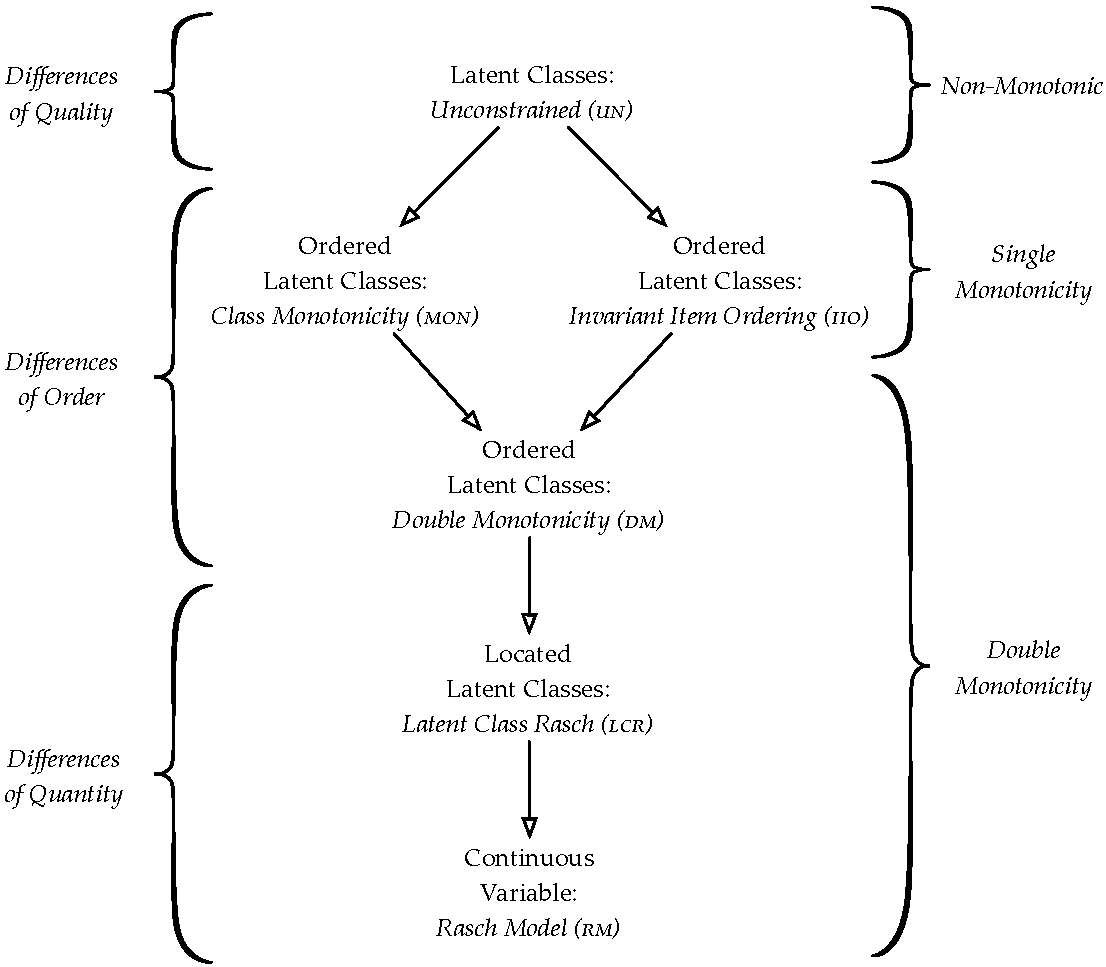
\includegraphics[width=0.75\textwidth]{./figs/Structure3.pdf} \\

\end{frame}


\section{Study design}

\begin{frame}
    \frametitle{Hypotheses}
    
    \parskip 12pt

    The expected order for the number of violations of the cancelation axioms is  
    \textsc{un} > ( \textsc{mon} $\sim$ \textsc{iio} ) > \textsc{dm} > ( \textsc{lcr} $\sim$ \textsc{rm} )

    \begin{center}
    \begin{tabular}{lccc}
    \toprule
     \multirow{3}{*}{Model} & \multicolumn{3}{c}{Violates cancelation axiom} \\ \cmidrule(lr){2-4}
                & \multicolumn{2}{c}{Single} & \multirow{2}{*}{Double} \\ \cmidrule(lr){2-3}
                  & Rows       & Columns    &            \\
    \midrule
     \textsc{un}  & \checkmark & \checkmark & \checkmark \\
     \textsc{mon} &            & \checkmark & \checkmark \\
     \textsc{iio} & \checkmark &            & \checkmark \\
     \textsc{dm}  &            &            & \checkmark \\
     \textsc{lcr} &            &            &            \\
     \textsc{rm}  &            &            &            \\
    \bottomrule
    \end{tabular}
    \end{center}

    If these hypotheses hold, then we potentially have a fairly straightforward criteria to recover the generating latent structure.

\end{frame}

\begin{frame}
    \frametitle{Simulation design and analysis}

        \begin{outline}
        \1 Generate data under each of six models 
        \renewcommand{\outlineii}{enumerate}
            \2 Use original data from Diakow and Torres Irribarra
                \3 5000 people in 2-6 classes
                \3 10 items
                \3 30 replications per model
            \2 Simulate new data 
                \3 1000 people in 6 classes
                \3 50 items in 6 groups
                \3 50 replications per model
        
        \vspace{0.25cm}
        
        \1 Check for violations of the cancelation axioms using ConjointChecks
        \renewcommand{\outlineii}{itemize}
            \2 Double cancelation and each single cancelation separately

        \vspace{0.25cm}

        \1 Record the \% of (weighted) violations for each model
    \end{outline}

\end{frame}


\section{Results}

\begin{frame}
    \frametitle{Simulation 1: Results for single cancelation}
        \framesubtitle{Person ordering}

    \centering 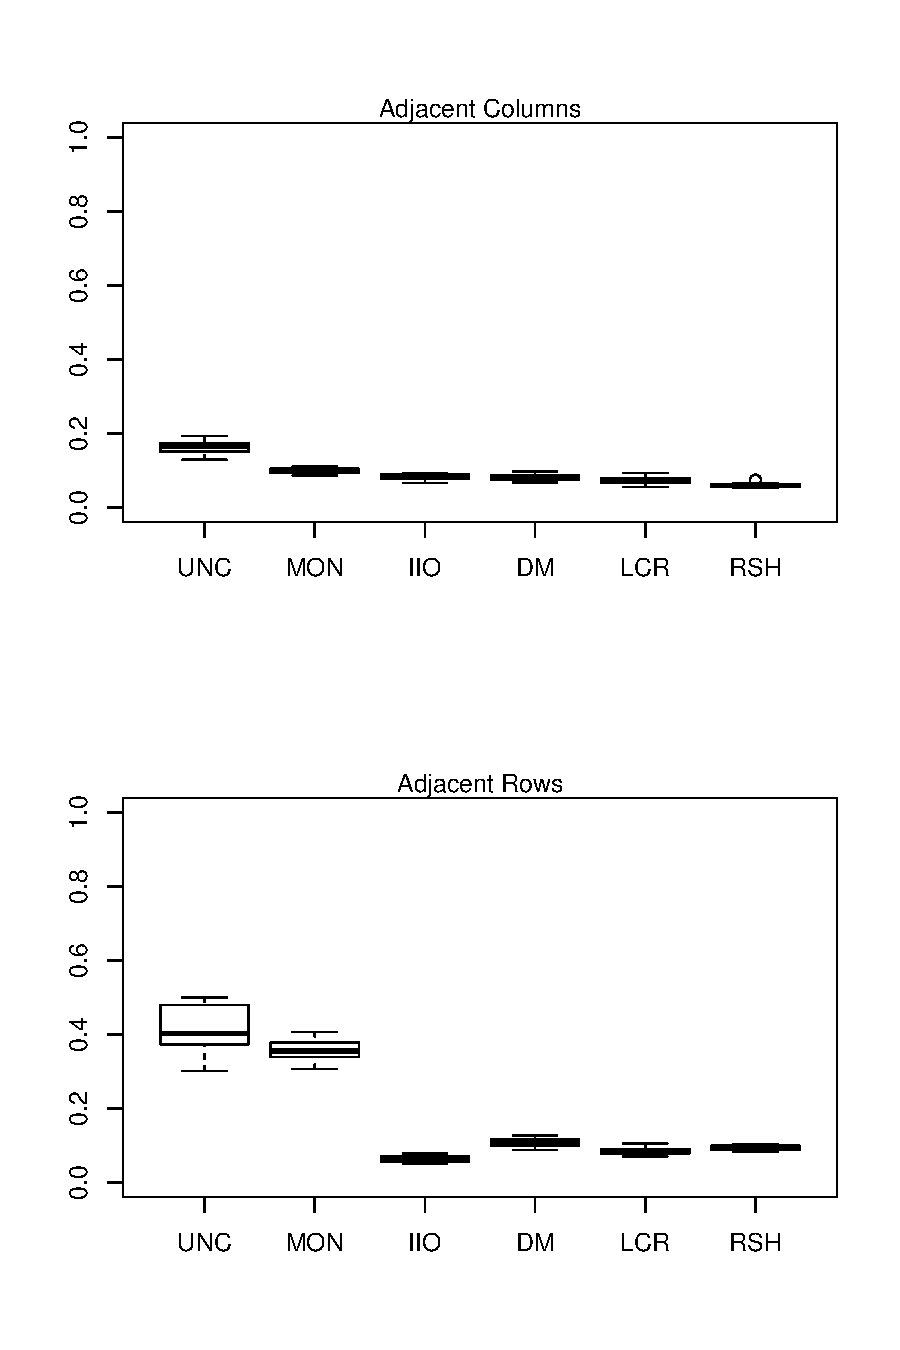
\includegraphics[width=0.75\textwidth, clip, trim = 0 4.5in 0 0]{./figs/boxplots_single.pdf}

\end{frame}

\begin{frame}
    \frametitle{Simulation 1: Results for single cancelation}
        \framesubtitle{Item ordering}

    \centering 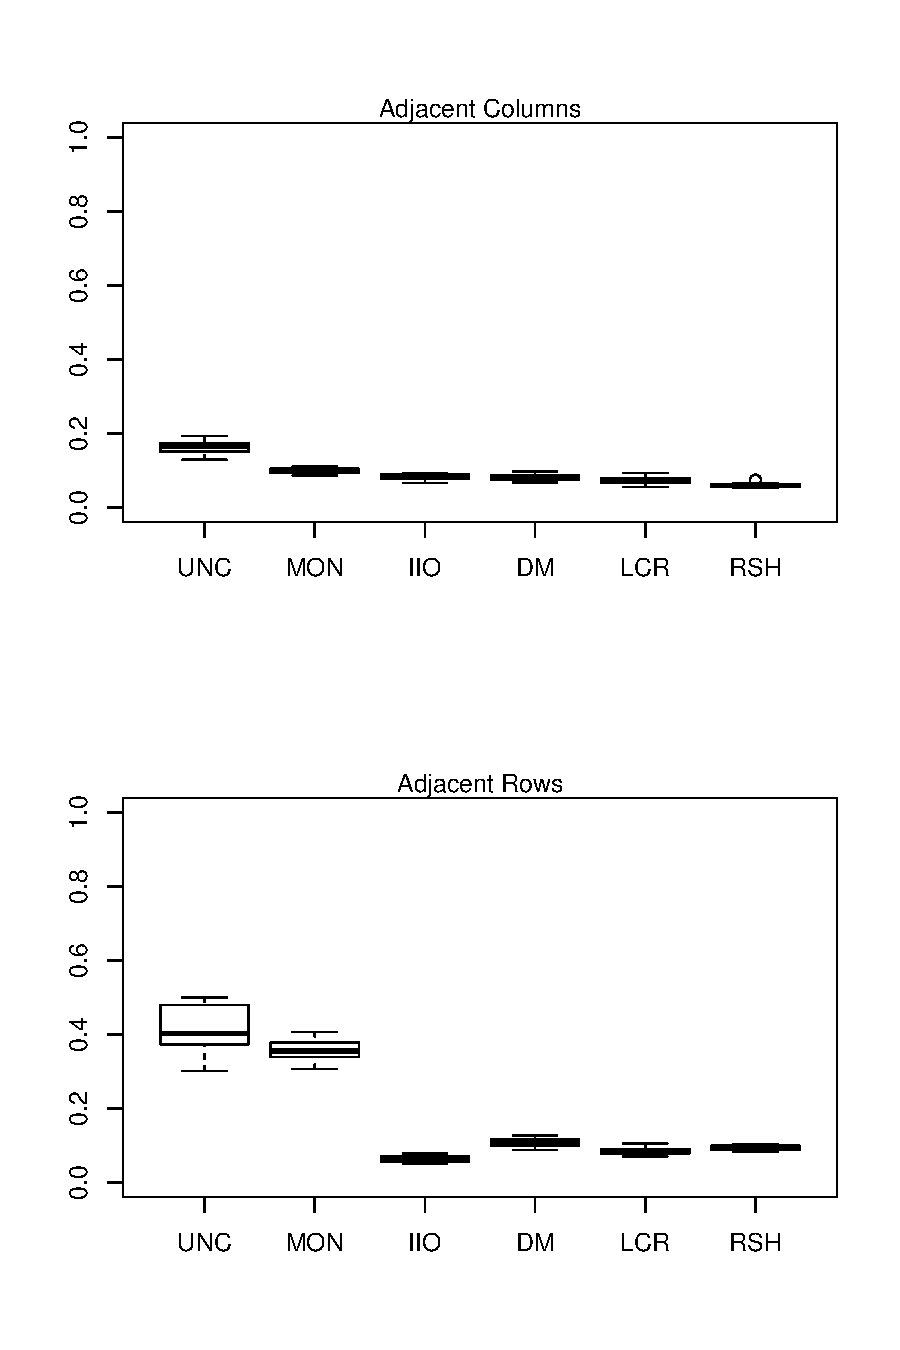
\includegraphics[width=0.75\textwidth, clip, trim = 0 0 0 4.5in]{./figs/boxplots_single.pdf}

\end{frame}

\begin{frame}
    \frametitle{Simulation 1: Results for double cancelation}

    \centering 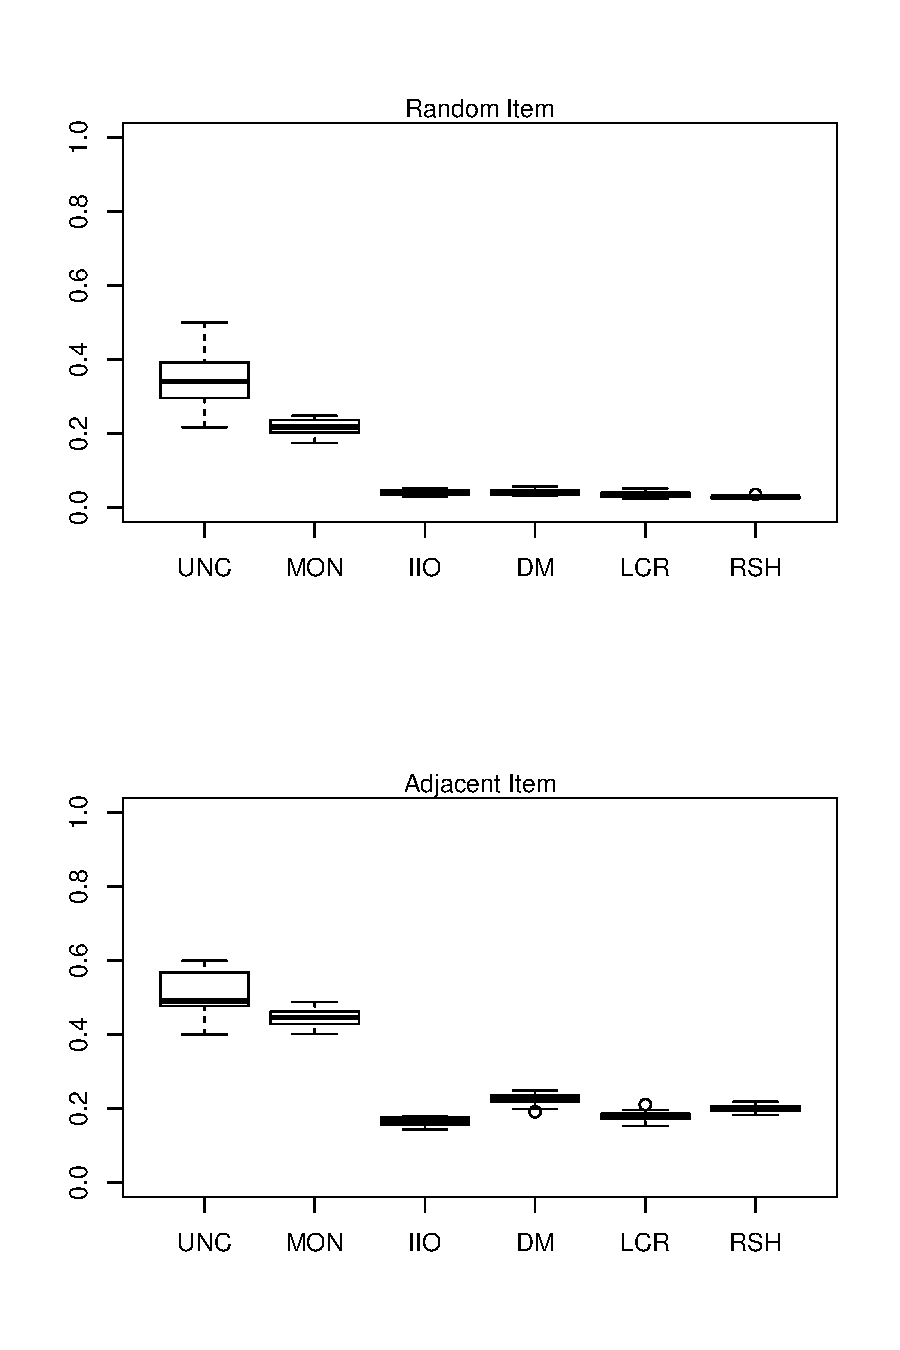
\includegraphics[width=0.75\textwidth, clip, trim = 0 0 0 4.5in]{./figs/boxplots.pdf}

\end{frame}


\begin{frame}
    \frametitle{Simulation 2: Single cancelation}
        \framesubtitle{Person ordering}

    \centering 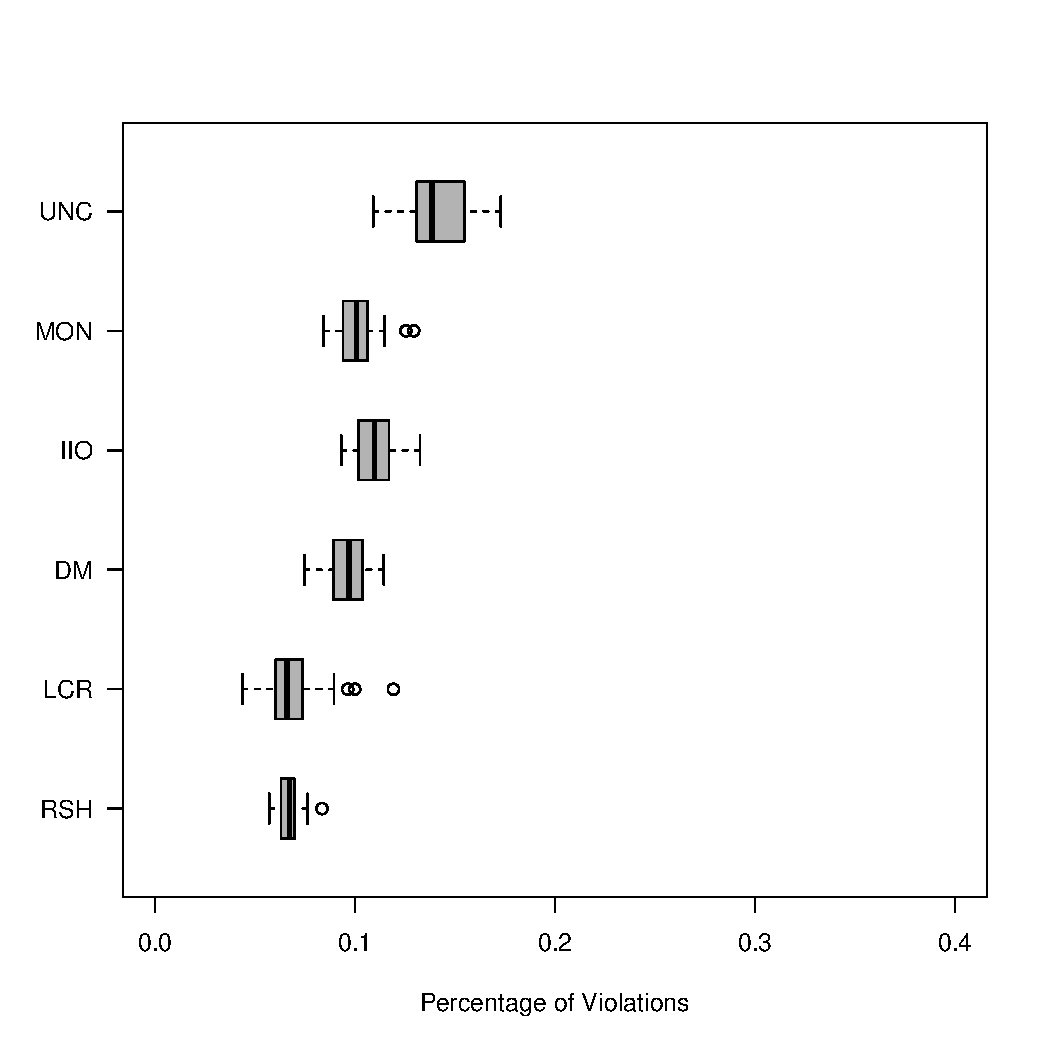
\includegraphics[width=0.75\textwidth]{./figs/violations_columns_weighted.pdf}

\end{frame}

\begin{frame}
    \frametitle{Simulation 2: Single cancelation}
        \framesubtitle{Item ordering}

    \centering 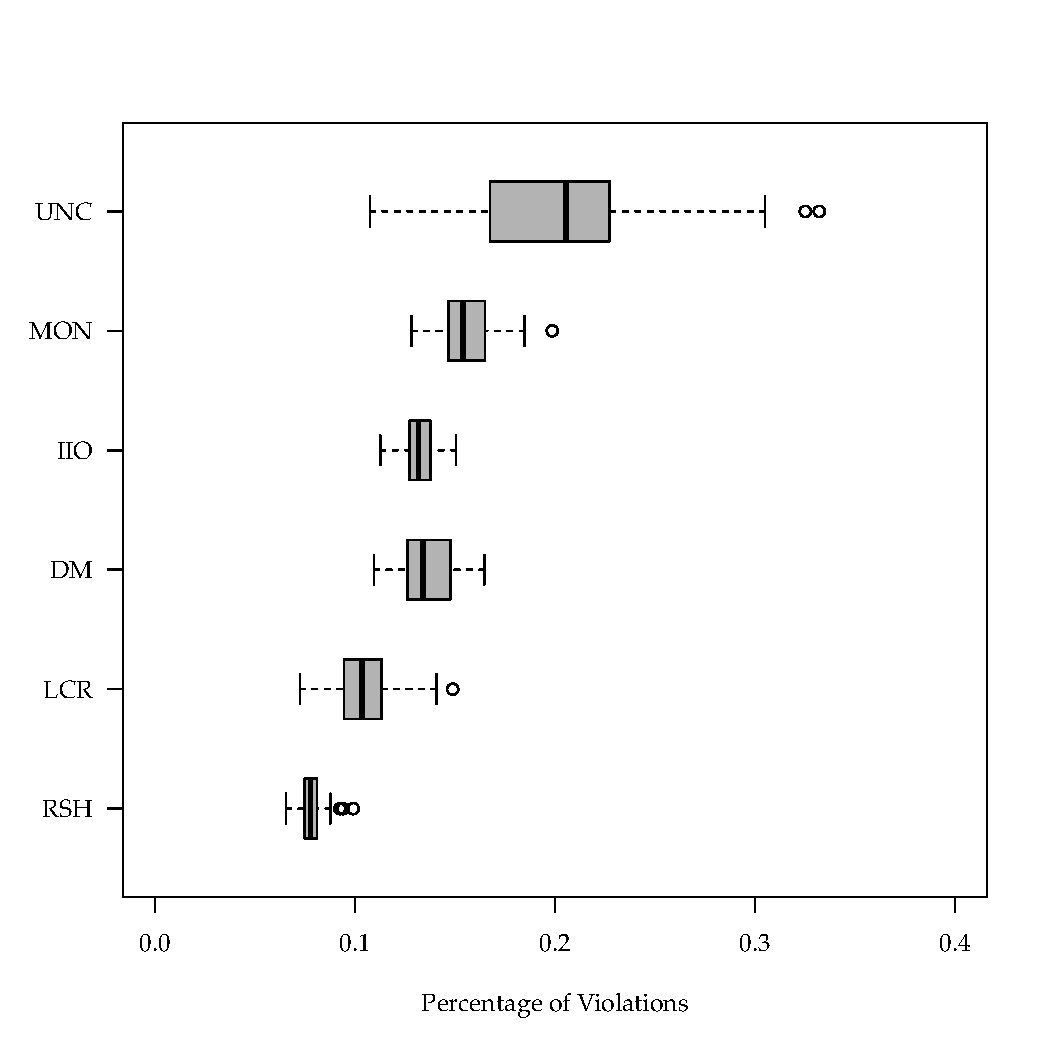
\includegraphics[width=0.75\textwidth]{./figs/violations_rows_weighted.pdf}

\end{frame}

\begin{frame}
    \frametitle{Simulation 2: Double cancelation}

    [include figure]

\end{frame}

\section{Discussion}

\begin{frame}
    \frametitle{Discussion}

    \begin{outline}
        \1 Person monotonicity versus item ordering
            \2 precision / aggregation
            \2 we don't usually treat persons and items as symmetric, though the models/checks formally do

        \1 Reconsidering double cancelation
            \2 standard testing data too noisy to check this?
    \end{outline}

\end{frame}

\begin{frame}
    \frametitle{Summary}
    
    \begin{outline}
        \1 
        
        \1 
        
        \1 
        
    \end{outline}

\end{frame}

\frame[contactinfo]{

    \begin{center}

    \Large Applying the Axioms of Additive Conjoint Measurement to a Hierarchy of Latent Variable Models

    \vspace{10mm}

    \small

    \begin{tabular}{rl}

        xxx@xxx.xxx          & \textsc{Benjamin Domingue} \\
        dti@berkeley.edu     & \textsc{David Torres Irribarra} \\
        rdiakow@berkeley.edu & \textsc{Ronli Diakow}

    \end{tabular}

    \end{center}

    \vspace{10mm}

%    \scriptsize
%    \hspace{5mm} Torres Irribarra, D., and Diakow, R.  (2011, July).  Model Selection for Tenable Assessment: Selecting a Latent Variable Model by Testing the Assumed Latent Structure.  Paper presented at the 76th Annual and 17th International Meeting of the Psychometric Society, Hong Kong.


}


%back-up slides
\appendix

%fix so slide numbering ignores back-up slides
\newcounter{finalpage}
\setcounter{finalpage}{\value{page}}
\newcounter{finalframe}
\setcounter{finalframe}{\value{framenumber}}
\setbeamertemplate{footline}{}

\begin{frame}

    \centering Appendix Slides

\end{frame}

%fix so slide numbering ignores back-ups
\setcounter{page}{\value{finalpage}}
\setcounter{framenumber}{\value{finalframe}}

\end{document}


\begin{frame}
    \frametitle{}

\end{frame} 